\chapter{Introduction}

Welcome to the world of "Linear Algebra and Analytic Geometry", a journey that unfolds the elegance and applicability of two foundational branches of mathematics. This book is designed to be your companion as you explore the intricacies of linear algebra and analytic geometry, essential disciplines that underpin a myriad of scientific and engineering applications.

\noindent
In this introduction, we set the stage for a comprehensive exploration of mathematical concepts that form the backbone of various fields. Linear algebra, with its rich tapestry of vector spaces, matrices and vector spaces, provides a versatile toolkit for problem-solving and modeling. Analytic geometry, the seamless integration of algebra and geometry, empowers us to visualize and analyze mathematical structures in a way that transcends abstract representation.

\noindent
As we embark on this journey, you will find a distinctive feature of this book: the integration of the powerful Python programming language. Python serves as our tool to bridge theory and practice, enabling you to implement and experiment with the concepts covered in a hands-on, interactive manner. Whether you are a student seeking a solid foundation or a practitioner aiming to refresh and deepen your knowledge, this book caters to a diverse audience with varying levels of expertise.

\noindent
The chapters ahead will guide you through the fundamental principles, practical applications, and real-world implications of linear algebra and analytic geometry. We will explore the interconnected nature of these subjects, providing not only theoretical insights but also practical skills that can be directly applied in scientific research, data science, computer engineering, and many other domains.

\noindent
The intersection of linear algebra and analytic geometry forms a rich tapestry where abstract mathematical structures meet real-world geometric representations. In Figure \ref{fig:conceptual-map}, a conceptual map visually encapsulates this symbiotic relationship, illustrating how vectors, matrices, and systems of linear equations seamlessly connect with geometric entities like lines, planes, and conics. Linear algebra provides the theoretical framework, offering tools to understand transformations and relationships among vectors. Simultaneously, analytic geometry provides a tangible canvas where these abstract principles manifest visually. This convergence enhances our ability to analyze spatial relationships, solve complex problems, and bridge the gap between mathematical abstraction and geometric reality.

\vspace{10pt}

\begin{figure}[h]
    \centering
    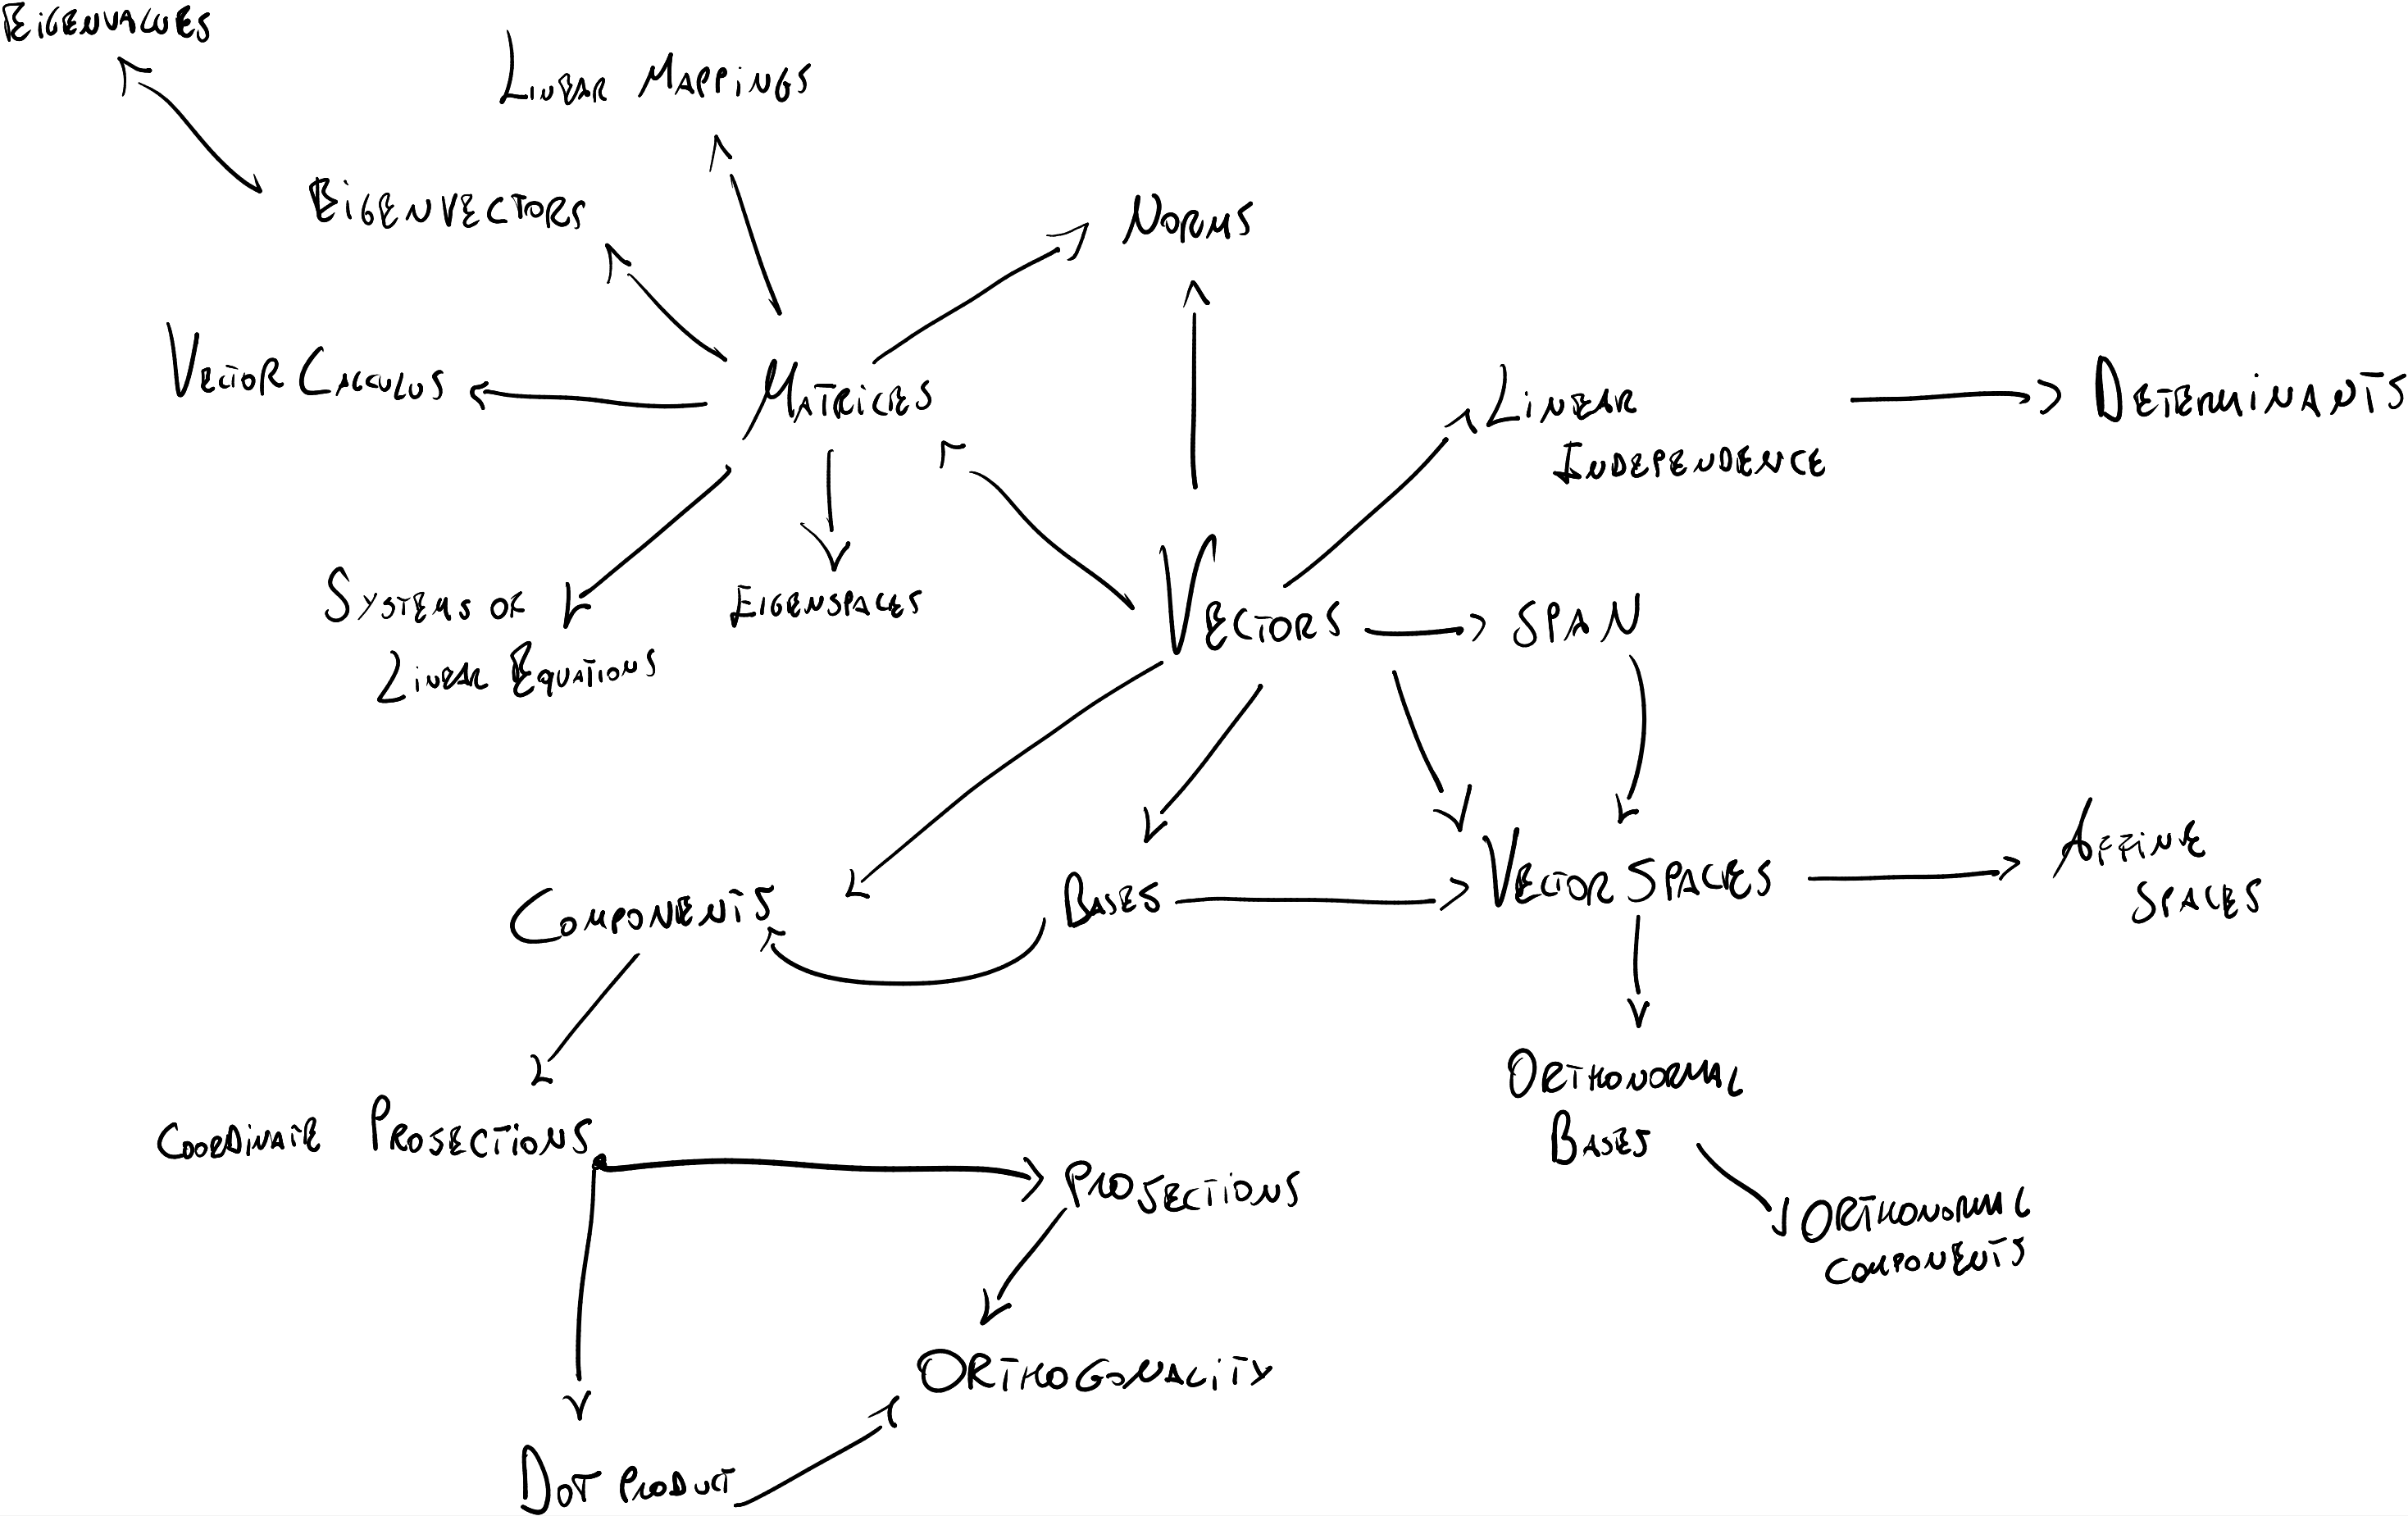
\includegraphics[scale=0.15]{Images/Linear_Algebra-map.png}
    \caption{Conceptual map of intersection of Linear Algebra and Analytic Geometry}
    \label{fig:conceptual-map}
\end{figure}

\noindent
Join me on this mathematical odyssey, where clarity, intuition, and computational prowess converge to make the abstract tangible. Let's unravel the beauty of linear algebra and analytic geometry, armed with the simplicity of Python programming, as we navigate through the pages of discovery and learning.

\section{Objects}
In the realm of mathematics, fundamental objects like scalars, vectors, matrices, and tensors serve as the building blocks for expressing a wide range of mathematical and scientific concepts. These entities encapsulate different levels of complexity, from singular values to multi-dimensional structures, each offering unique properties and applications.

\subsection{Scalars}
Scalars are elements of a field, like $\mathbb{R}$,that represent quantities that only have magnitude, such as temperature, mass, distance, or time. Scalars have zero dimensions. They are considered point values in a mathematical space.

Since a scalar has no dimensions, its shape is represented as an empty set.

Scalars are typically denoted by lowercase letters, e.g., $a,b,c$ and they are treated as constants; they can be real numbers, complex numbers, or elements from other mathematical fields.
\\

For example 

$$
a \in \mathbb{F}
$$

where is a scalar in a field $\mathbb{F}$.

\subsection{Vectors}
A vector is an ordered collection of elements of a field that represents a quantity with both magnitude and direction. Vectors are used to describe various physical quantities, such as displacement, velocity, and force.
In a geometric sense, they can be visualized as directed line segments with a specific length and direction in space.

Vectors have one dimension, so the shape of a vector is a 1-dimensional tuple $(n)$, where $n$ is the number of elements in the vector, also known as vector size. 
\\

Here are a few key points to understand about vectors:
\begin{itemize}
    \item \textbf{Magnitude:} This is the length of the vector.

    \item \textbf{Direction:} This indicates the way the vector points.

    \item \textbf{Components:} The individual parts that make up a vector.
\end{itemize}

They are typically denoted by a letter with an arrow above. For example

$$
\vec v =\begin{bmatrix}
    v_1\\
    v_2\\
    \vdots\\
    v_n
\end{bmatrix} \in \mathbb{F}^n,
$$

where $\vec v$ is a vector in $\mathbb F^n$, $(n)$ is the vector shape, $n$ is the vector size and $v_1, v_2, \dots, v_n \in \mathbb{F}$ are vector components.

If we wish to access the component within the vectors we can employ the following mathematical notation: 

$$
\vec v^{\ (1)} = v_1
$$

And to access all elements of a dimension we can use ":" instead of numerical indexes:

$$
\vec v^{\ (:)} = \vec v
$$

\subsection{Matrices}
A matrix is a two-dimensional array of elements of a field, organized in rows and columns. It is used to represent and manipulate data in various applications, including linear transformations and systems of equations.

The shape of a matrix is a 2-dimensional tuple $(m,n)$, where $m$ is the number of rows and $n$ is the number of columns. 

Matrices are typically denoted by uppercase letters, e.g., $A, B, C$. For example 

$$
A_{m,n} = \begin{bmatrix} 
    a_{11} & \dots  & a_{1n}\\
    \vdots & \ddots & \vdots\\
    a_{m1} & \dots  & a_{mn} 
\end{bmatrix} \in \mathbb{F}^{m \times n}
$$

where $A_{m,n}$ is a matrix in $\mathbb{F}^{m \times n}$, $(m, n)$ is the matrix shape and $a_{i,j} \in \mathbb F$.

If we wish to access the component within the matrix we can employ the following mathematical notation: 

$$
A_{m,n}^{(i, j)} = a_{i,j}
$$

And to access all elements of a dimension we can use ":" instead of numerical indexes:

$$
A_{m,n}^{(i, :)} = \begin{bmatrix}
    a_{i,1}\\
    a_{i, 2}\\
    \vdots\\
    a_{i, n}
\end{bmatrix}, \quad A_{m,n}^{(:, j)} = \begin{bmatrix}
    a_{1,j}\\
    a_{2,j}\\
    \vdots\\
    a_{m,j}
\end{bmatrix}, \quad  A_{m,n}^{(:, :)} = A_{m,n}
$$


\subsubsection{Square Matrices}

A square matrix $A_{m,n}$ is a matrix with the same number of rows and columns, i.e., $m = n$.

\subsubsection{Triangular Matrices}
A lower triangular matrix $A$ is a square matrix where all entries above the main diagonal are zero, i.e., $a_{i,j} = 0$ for $i < j$.

An upper triangular matrix $A$ is a square matrix where all entries below the main diagonal are zero, i.e., $a_{i,j} = 0$ for $i > j$.

\subsubsection{Diagonal Matrices}

A diagonal matrix $D$ is a square matrix where all entries outside the main diagonal are zero, i.e., $a_{i,j} = 0$ for $i \neq j$.

\subsubsection{Symmetric Matrices}
A symmetric matrix $A_{n,n}$ is a square matrix where the elements are symmetric with respect to the main diagonal. 
In other words, if $a_{i,j}$ is an entry in the matrix at the $i$-th row and $j$-th column, then $a_{i,j} = a_{j,i}$ 
for all $i$ and $j$ in the matrix. This symmetry implies that the values on one side of the main diagonal mirror the 
values on the other side.

% Diagonale di una matrice
%%Null matrix
\section{Basic Operations}
In the world of linear algebra, basic operations form the cornerstone of mathematical manipulations applied to our objects (scalar, vectors and matrices). These operations serve as fundamental tools for analyzing and transforming these mathematical entities, unlocking insights across various disciplines.

\subsection{Transposition}

In linear algebra, transposition refers to the operation of switching the rows and columns of a mathematical object. This operation is commonly applied to matrices, and geometrically can be interpreted as reflecting the matrix over its main diagonal.

\subsubsection{Matrices Transposition}

For a given matrix $A_{m,n} \in \mathbb F^{m \times n}$, the transpose, denoted as $A_{m,n}^T$, is obtained by swapping its rows with columns. Mathematically, each $a_{i,j}$ in $A_{m,n}$, would be mapped into $a_{ji}$. In other words, the element in the $i$-th row and $j$-th column of $A_{m,n}^T$ is the same as the element in the $j$-th row and $i$-th column of $A_{m,n}$.

So $A_{m,n}^T = A_{n,m}'$.
\\

\textbf{Example:}

Consider the following matrix:
\[
A = \begin{bmatrix}
    1 & 2 & 3 \\
    4 & 5 & 6 \\
    7 & 8 & 9 \\
\end{bmatrix}
\]

The transpose of matrix $A$ is:
\[
A^T = \begin{bmatrix}
    1 & 4 & 7 \\
    2 & 5 & 8 \\
    3 & 6 & 9 \\
\end{bmatrix}
\]

\subsubsection{Properties:}

\begin{itemize}
    \item $(A^T)^T = A$: Transposing a matrix twice results in the original matrix.
    \item $(cA)^T = cA^T$: Transposing a scaled matrix is equivalent to scaling the transpose.
    \item $(A + B)^T = A^T + B^T$: Transposing the sum of two matrices is equivalent to the sum of their transposes.
\end{itemize}

These properties are fundamental in various mathematical applications, including linear algebra and optimization.


\subsection{Addition}
In linear algebra, the sum of two objects is a fundamental operation that combines their respective components.
We are very familiar with the common sum of scalars:

$$
a + b = c,
$$
but what happens when we need to apply the sum to objects of dimension greater than 0?
\\

Vector sum, for example is defined as follow. 
\\

Let 
$$
\vec{v} = \begin{bmatrix} v_1 \\ v_2 \\ \vdots \\ v_n \end{bmatrix}, \quad \vec{w} = \begin{bmatrix} w_1 \\ w_2 \\ \vdots \\ w_n \end{bmatrix}
$$
be two vectors in \(\mathbb{F}^n\). 
    The sum of two vectors \(\vec{v}\) and \(\vec{w}\), denoted as \(\vec{v} + \vec{w}\), is defined component-wise:
    
\[ \vec{v} + \vec{w} = \begin{bmatrix} v_1 + w_1 \\ v_2 + w_2 \\ \vdots \\ v_n + w_n \end{bmatrix} \]

Geometrically, vector addition corresponds to placing the initial point of the second vector at the terminal point of the first vector and connecting the initial point of the first vector to the terminal point of the second vector (as shown in Figure \ref{fig:vector-sum-1}).
\\
\begin{figure}[h]
    \centering
    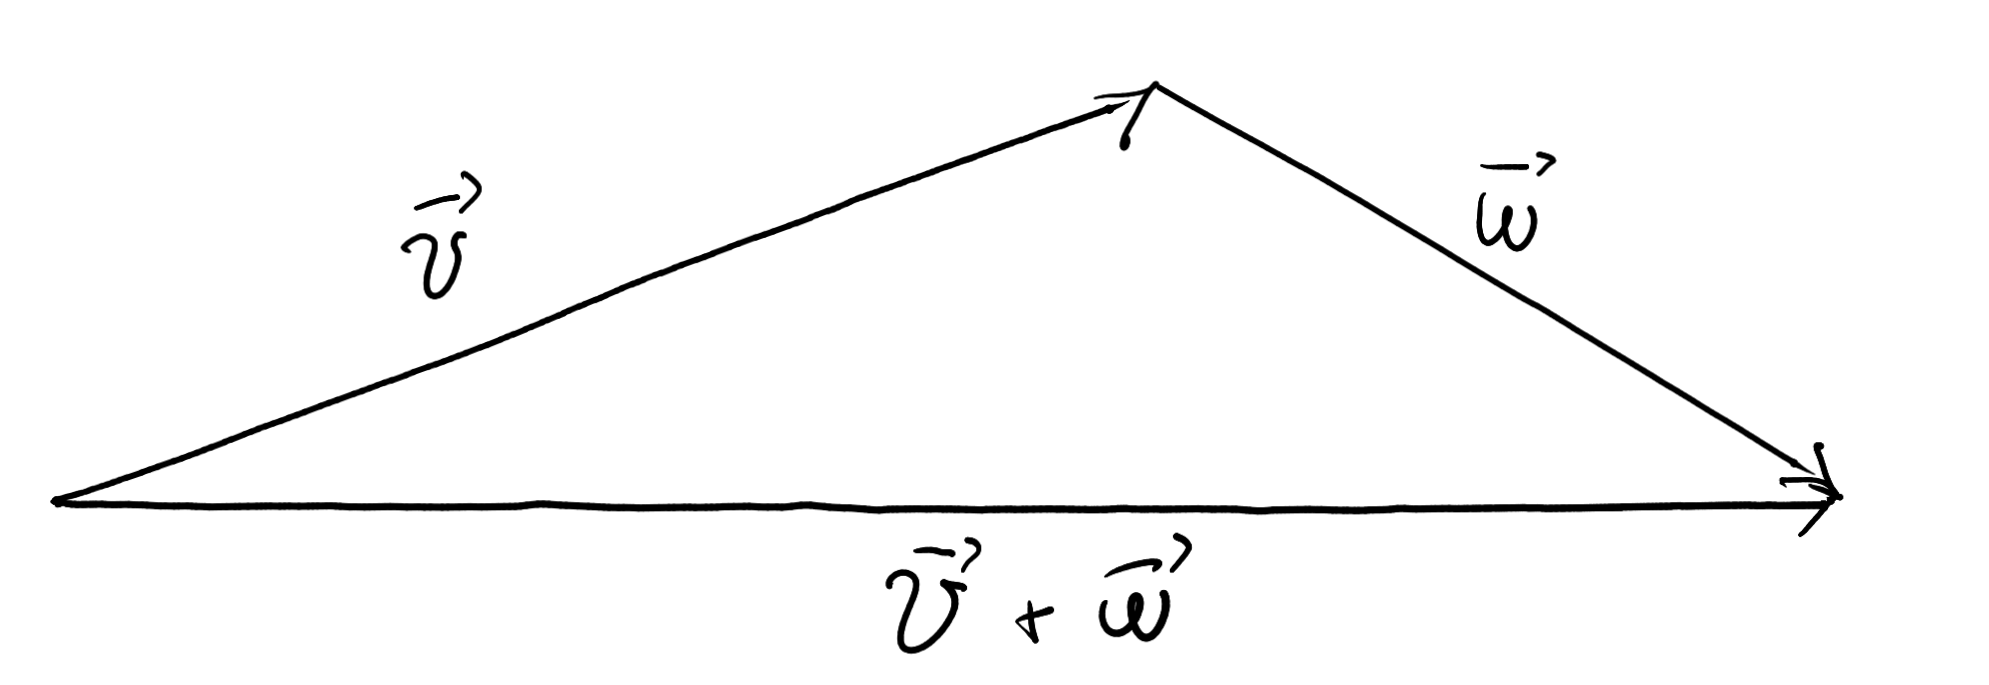
\includegraphics[scale=0.2]{Images/Linear_Algebra-vector-sum1.png}
    \caption{Triangle Law of Vector Addition}
    \label{fig:vector-sum-1}
\end{figure}

Now, let's consider an example of vector addition using two real vectors, $\vec a$ and $\vec b$. The sum of $\vec a$ and $\vec b$ will be:

$$
\vec a = \begin{bmatrix}
    1 \\
    2
\end{bmatrix}
\quad
\vec b = \begin{bmatrix}
    2 \\
    -3
\end{bmatrix}
$$

$$
\vec a + \vec b = \begin{bmatrix}
    a_0 + b_0 \\
    a_1 + b_1
\end{bmatrix} = \begin{bmatrix}
    1 + 2 \\
    2 + (-3)
\end{bmatrix} = \begin{bmatrix}
    3 \\
    -1
\end{bmatrix}
$$

\begin{figure}[h]
    \centering
    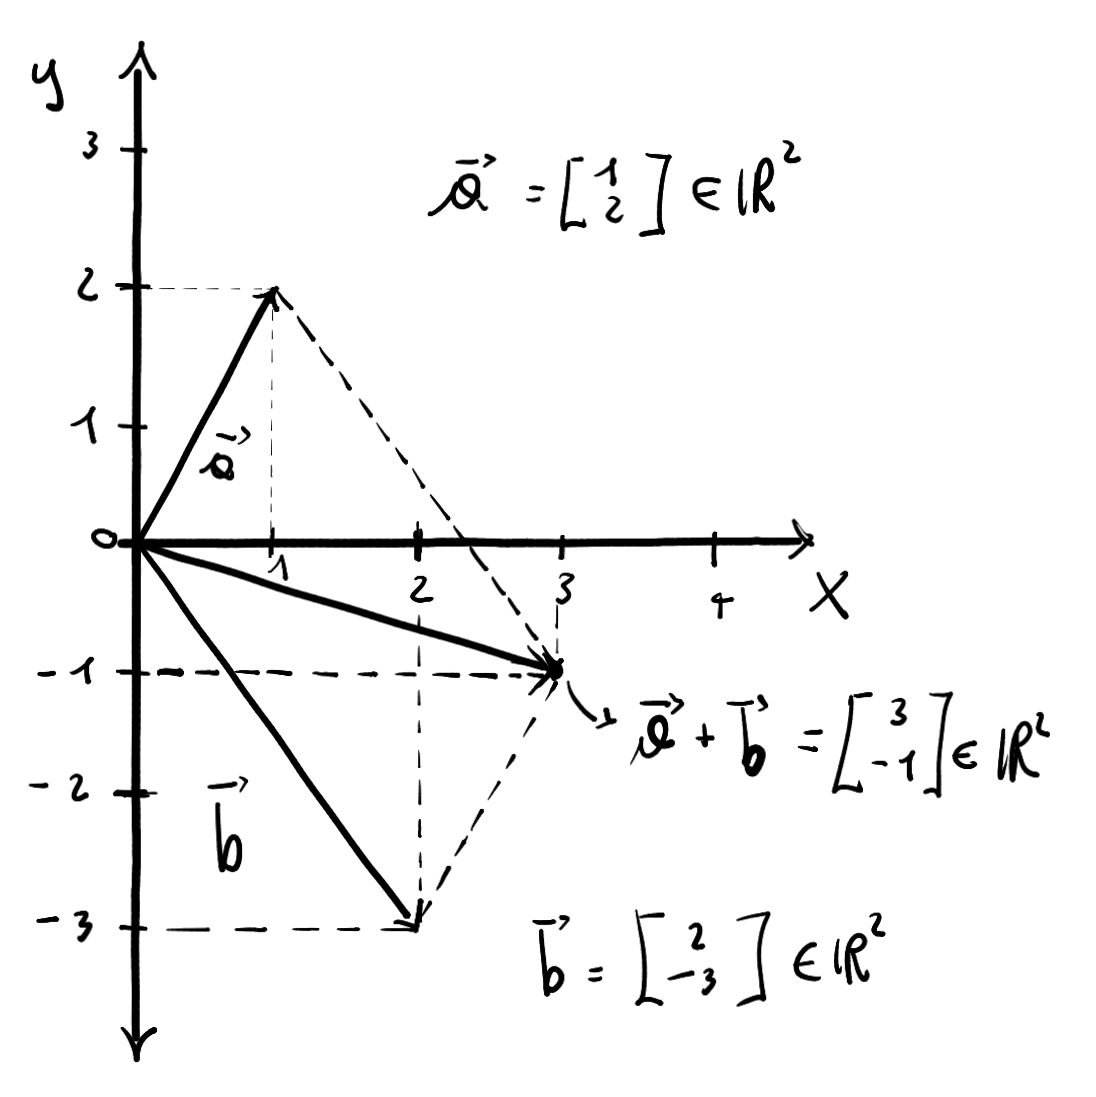
\includegraphics[scale=0.25]{Images/Linear_Algebra-vector-sum2.png}
    \caption{Parallelogram Law of Addition of Vectors}
    \label{fig:vector-sum-2}
\end{figure} 

The Figure \ref{fig:vector-sum-2} shows the vector sum graphically by using the Parallelogram law.

Note that we can sum together only vectors that have the same shape.
\\

The same concept can be applied to matrices, in fact given two matrices 

$$
A_{m,n} = \begin{bmatrix}
    a_{1,1} & a_{1,2} & \dots & a_{1,n} \\
    a_{2,1} & a_{2,2} & \dots & a_{2,n} \\
    \vdots & \vdots & \ddots & \vdots \\
    a_{m,1} & a_{m,2} & \dots & a_{m,n}
\end{bmatrix}, \quad
B_{m,n} = \begin{bmatrix}
    b_{1,1} & b_{1,2} & \dots & b_{1,n} \\
    b_{2,1} & b_{2,2} & \dots & b_{2,n} \\
    \vdots & \vdots & \ddots & \vdots \\
    b_{m,1} & b_{m,2} & \dots & b_{m,n}
\end{bmatrix}
$$

their sum is defined as

\[
A_{m,n} + B_{m,n} =
\begin{bmatrix}
    a_{1,1} + b_{1,1} & \dots & a_{1,n} + b_{1,n} \\
    a_{2,1} + b_{2,1} & \dots & a_{2,n} + b_{2,n} \\
    \vdots & \ddots & \vdots \\
    a_{m,1} + b_{m,1} & \dots & a_{m,n} + b_{m,n}
\end{bmatrix}
=
\begin{bmatrix}
    c_{1,1} & \dots & c_{1,n} \\
    c_{2,1} & \dots & c_{2,n} \\
    \vdots & \ddots & \vdots \\
    c_{m,1} & \dots & c_{m,n}
\end{bmatrix}
= C_{m,n}
\]

or, more mathematically, the generic $c_{i,j}$ of $C_{m,n}$ of new matrices is equal to $a_{i,j} + b_{i,j}$.
Note that we can sum together only matrices that have the same shape.
\\

\subsection{Sum Over Axes}\label{subsection:sum-over-axes}
Now, let's introduce the concept of \textit{sum over axes}.

The \textit{sum over axes} operation plays a crucial role, particularly when dealing with high dimensionality objects. This operation allows us to efficiently contract algebraic objects along specified axes, resulting in a new object with reduced dimension.

Consider a very simple example, imagining having a vector $\vec{v} \in \mathbb{F}^n$ and wanting to perform a \textit{sum over axes} on its (only) axis, i.e., axis 0.

$$
\vec{v} = \begin{bmatrix}
    v_1 \\
    v_2 \\
    \vdots\\
    v_n
\end{bmatrix} \in \mathbb{F}^n \quad \underset{\text{Sum over 0 axis}}{\longrightarrow} = \sum_{i=0}^n v_i
$$

After the sum over the 0 axis of the vector $\vec{v}$, we obtain a scalar belonging to the same field as the vector components. 
\\

So, for example:

\[
\vec{v} = \begin{bmatrix}
    1 \\
    2 \\
    3
\end{bmatrix} \in \mathbb{F}^3 \quad \underset{\text{Sum over 0 axis}}{\longrightarrow} 
\begin{bmatrix}
    1 + 2 + 3
\end{bmatrix} = 6 \in \mathbb{F}
\]

Consider another very simple example, imagining having a matrix $A_{m,n}$ and wanting to perform a \textit{sum over axes} on axis 0.

$$
A_{m,n} = \begin{bmatrix}
    a_{1,1} & a_{1,2} & \dots & a_{1,n} \\
    a_{2,1} & a_{2,2} & \dots & a_{2,n} \\
    \vdots & \vdots & \ddots & \vdots \\
    a_{m,1} & a_{m,2} & \dots & a_{m,n}
\end{bmatrix}  \in \mathbb{F}^{m \times n} \quad \underset{\text{Sum over 0 axis}}{\longrightarrow} A_{1, n}' = 
\begin{bmatrix}
    \sum_{i=0}^m a_{i,1} & \sum_{i=0}^m a_{i,2} & \dots & \sum_{i=0}^m a_{i,n}
\end{bmatrix}
$$

For example:

\[
A_{3,4} = \begin{bmatrix}
    1 & 2 & 3 & -8 \\
    2 & 5 & -1 & 9 \\
    3 & 3 & -7 & -2
\end{bmatrix} \in \mathbb{F}^{3 \times 4} \quad \underset{\text{Sum over 0 axis}}{\longrightarrow} A_{1, 4}' = 
\begin{bmatrix}
    1 & 2 & 3 & -8 \\
    + & + & + & + \\
    2 & 5 & -1 & 9 \\
    + & + & + & + \\
    3 & 3 & -7 & -2
\end{bmatrix}
=
\begin{bmatrix}
    6 & 10 & -5 & -1
\end{bmatrix}
\]

Thus, we have obtained the \textit{sum over axes} on axis 0 of the matrix $A_{5,4}$, obtaining a row vector $A'$ of one dimension and size 4.

Similarly, if we wanted to perform a \textit{sum over axes} on axis 1, we would get

$$
A_{mn} = \begin{bmatrix}
    a_{1,1} & a_{1,2} & \dots & a_{1,n} \\
    a_{2,1} & a_{2,2} & \dots & a_{2,n} \\
    \vdots & \vdots & \ddots & \vdots \\
    a_{m,1} & a_{m,2} & \dots & a_{m,n}
\end{bmatrix} \in \mathbb{F}^{m \times n} \quad \underset{\text{Sum over 1 axis}}{\longrightarrow} A_{m, 1}' =
\begin{bmatrix}
    \sum_{i=0}^n a_{1,i} \\
    \sum_{i=0}^n a_{2,i} \\
    \vdots\\
    \sum_{i=0}^n a_{m,i}
\end{bmatrix}
$$
For example:
\[
A_{3,4} = \begin{bmatrix}
    1 & 2 & 3 & -8 \\
    2 & 5 & -1 & 9 \\
    3 & 3 & -7 & -2
\end{bmatrix} \in \mathbb{F}^{3 \times 4} \quad \underset{\text{Sum over 1 axis}}{\longrightarrow} A_{3, 1}' = 
\begin{bmatrix}
    1 + 2 + 3 - 8 \\
    2 + 5 - 1 + 9 \\
    3 + 3 - 7 - 2
\end{bmatrix}
=
\begin{bmatrix}
    -2 \\
    15 \\
    -3
\end{bmatrix}
\]


\subsection{Multiplication}
When we talk about product, we are, of course, referring to the multiplication between two algebraic objects. When these two objects are scalars, we don't need to consider the issue of dimensionality, as scalars are objects with no dimension, and therefore, their product will inevitably have no dimension. However, as the complexity (and hence, dimension) of the objects we want to multiply increases and differs between the two objects, we need to take into account not only the product itself, but also the dimensional differences involved. In fact, as the shape of the objects increases (and differs), the possible ways of performing their product also increase.

In the following sections, it will become clearer in what ways it is possible to perform the standard product between two objects (scalar, vectors or matrices) and what is the difference with standard product, \textbf{Hadamard} product and \textbf{Kronecker} product.

Esistono molti modi di calcolare il prodotto tra due ogetti algebrici, ma la caratteristica che li accomuna è che tutti i prodotti si basano su due operazioni fondamentali:

\begin{itemize}
    \item Sum over axes.
    \item Moltiplicazione tra scalari.
\end{itemize}

Dove la \textit{sum over axes}, precedentemente introdotta nella sottosezione \ref{subsection:sum-over-axes}, ci permette di eseguire le operazioni di contrazione degli assi necessarie al calcolo del prodotto di due ogetti algebrici.

Mentre il prodotto standard tra scalari è il normale prodotto a cui siamo abituati; definito per due generici elementi $a, b$ del campo $\mathbb{F}$ come:

$$
a \cdot b = c \in \mathbb{F}
$$

Tramite queste due operazioni siamo in grado di eseguire il prodotto di due elementi algebrici di dimensionalità arbitraria.

\subsubsection{Compatibilità tra Assi}

Prima di addentrarci nel calcolo vero e proprio, dobbiamo chiarire anche un altro punto, senza il quale non è possibile eseguire tutte le tipologie di prodotto. Introduciamo quindi il concetto di \textit{compatibilità tra assi}: due assi (dimensioni) si dicono compatibili se e solo se hanno la stessa size (contengono lo stesso numero di elementi). Per asse si intende la dimensione, ad esempio l'asse 0 (l'unico) del vettore $\vec v \in  \mathbb{F}^n$ è la sua dimensione, l'asse del vettore $\vec w \in \mathbb{F}^m$ sono compatibili se e solo se $n = m$. 

Facciamo un altro esempio, siano $A_{3, 2} \in \mathbb{F}^{3 \times 2}$ e $B_{2, 3} \in \mathbb{F}^{2 \times 3}$ due matrici, in questo caso l'asse 0 della matrice $A_{3,2}$ e l'asse 1 della matrice $B_{2, 3}$ sono compatibili, ma anche l'asse 1 della matrice $A_{3,2}$ e l'asse 0 della matrice $B_{2,3}$ lo sono.

Mentre eseguiamo il prodotto di due ogetti algebrici, può essere necessario tenere conto di quali assi sono compatibili, perchè alcuni tipi di prodotto necessitano tale requisito.

\subsubsection{Prodotto}
In generale il prodotto tra due generici ogetti algebrici viene calcolato attraverso una prima fase di scelta degli assi compatibili sui quali effettuare la contrazione, e una seconda fase nella quale si effettua il broadcast sulle dimensioni che non sono state scelte per la contrazione. In generale il risultato è dato da un ogetto che ha per dimensioni tutte le dimensioni "non scelte" in ordine di moltiplicazione. 

In questa sezione ci limiteremo a descrivere le principali metodologie di calcolo del prodotto.
\\
 
L'esempio più semplice (escluso il prodotto tra scalari) è il prodotto di uno scalare per un vettore. In questo caso non si scelgono assi compatibili (perché non ve ne sono) quindi non si effettua la contrazione, ma si passa direttamente alla fase di broadcast dello scalare per ogni componente del vettore. Tale prodotto è definito tra uno scalare $a \in \mathbb F$ e un vettore $\vec v \in \mathbb{F}^n$ e si scrive

$$
a \cdot \vec v = a \cdot \begin{bmatrix}
    v_1\\
    v_2\\
    \vdots\\
    v_n
\end{bmatrix} = \begin{bmatrix}
    a \cdot v_1\\
    a \cdot v_2\\
    \vdots\\
    a \cdot v_n
\end{bmatrix} \in \mathbb F^{n}.
$$

Il risultato è un vettore con la stessa size del vettore moltiplicato. Infatti se prendiamo la shape dello scalare $()$ e la shape del vettore $(n)$ e le mettiamo insieme otteniamo la shape del vettore risultato, che, dato che lo scalare non ha dimensioni, è proprio $(n)$.
\\
\iffalse
Facciamo però un esempio concreto: siano $\vec v = \beg$
\begin{figure}[h]
    \centering
    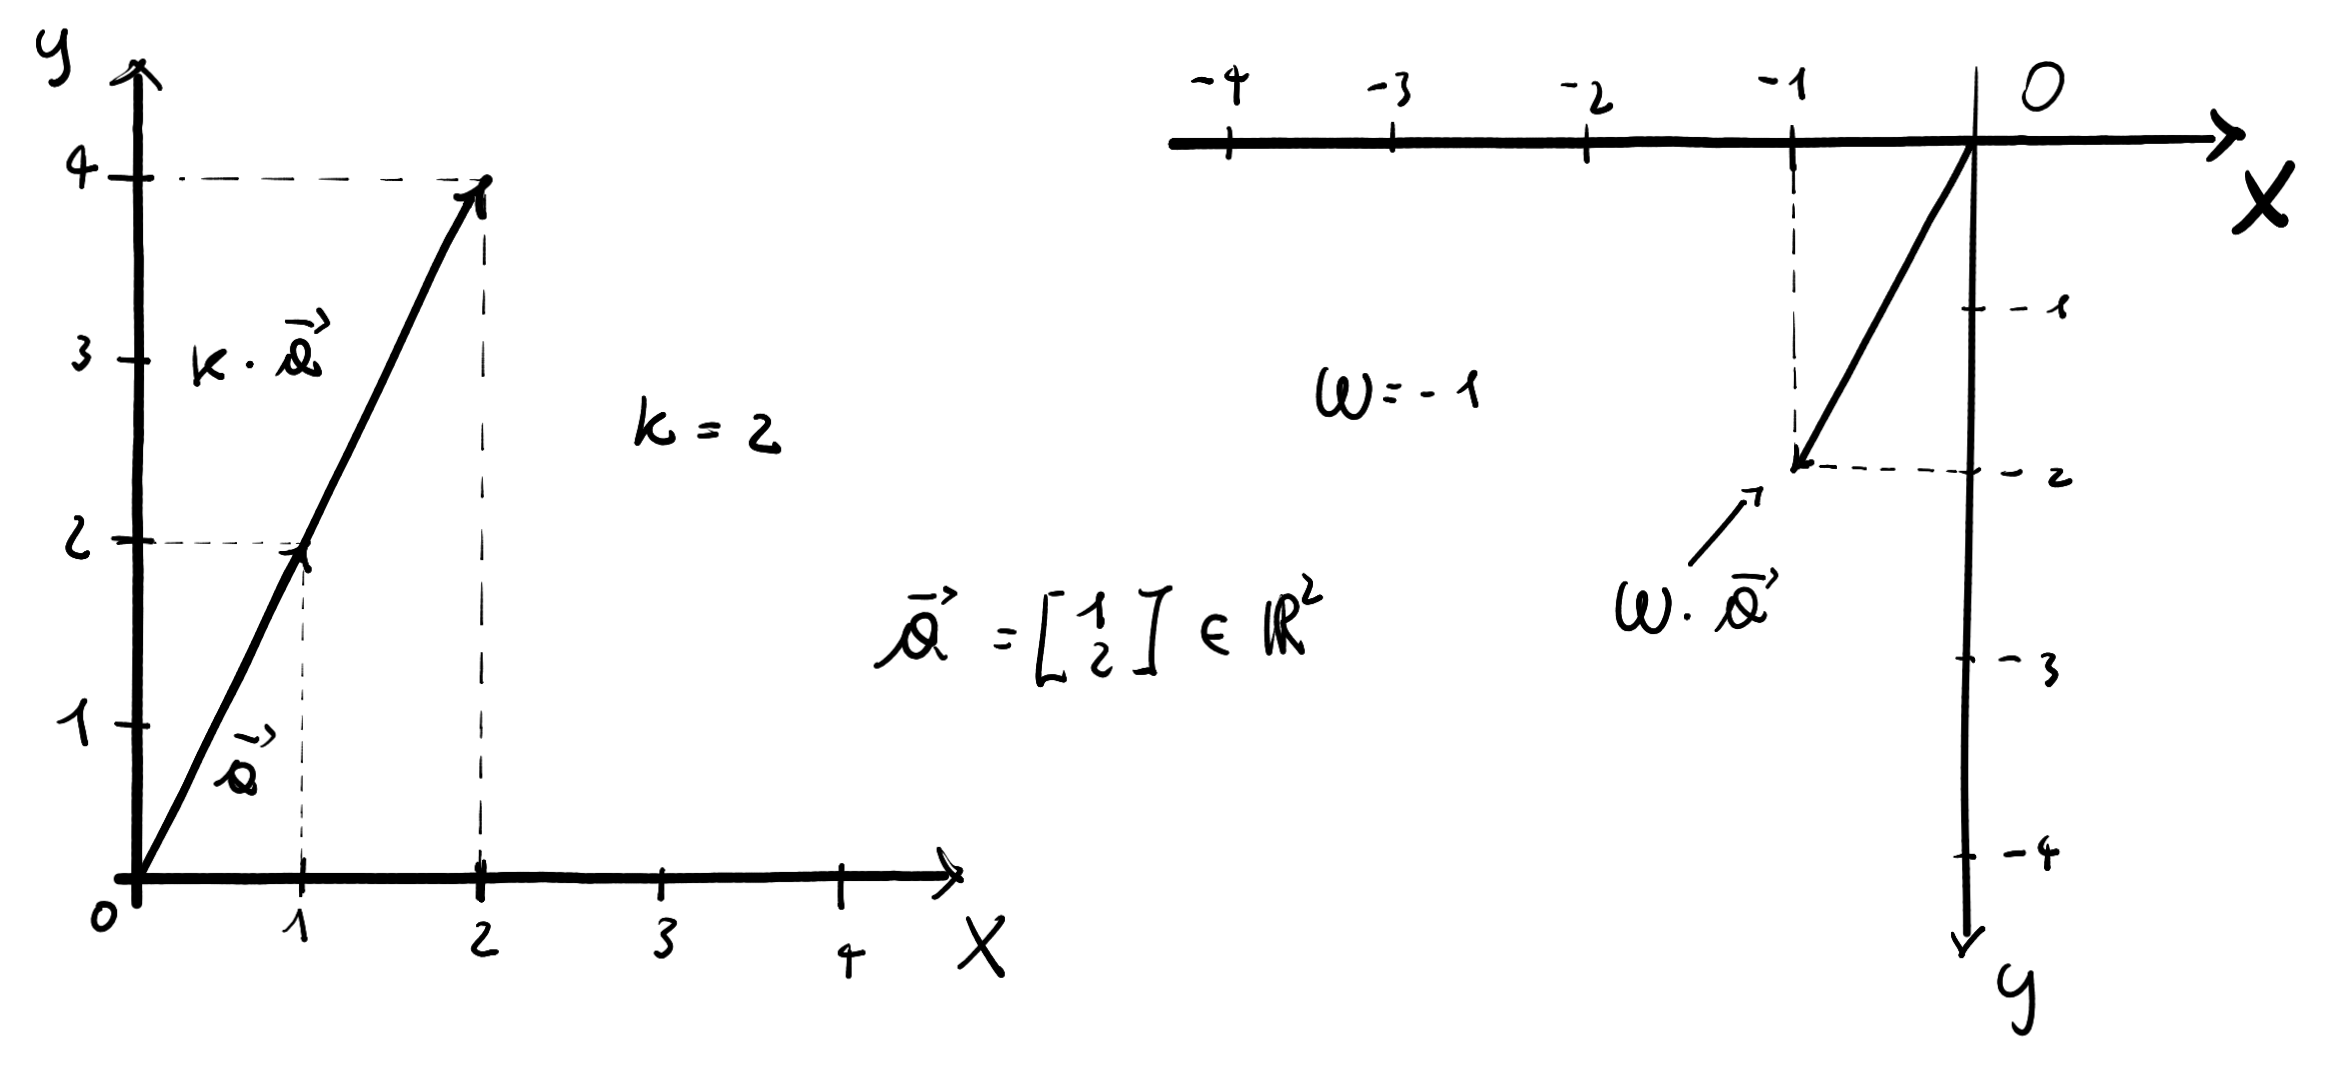
\includegraphics[scale=0.18]{Images/Linear_Algebra-scalar-mul.png}
    \caption{}
    \label{fig:scalar-mul}
\end{figure} 
\fi

Allo stesso modo, il prodotto tra uno scalare $a \in \mathbb F$ e una matrice $B_{m,n} \in\mathbb F^{m \times n}$ è definito come 

$$
a \cdot B_{m,n} = a \cdot \begin{bmatrix}
    b_{1,1} & \dots & b_{1,n}\\
    b_{2,1} & \dots & b_{1,n}\\
    \vdots  & \ddots & \vdots \\
    b_{m,1} & \dots & b_{m,n}
\end{bmatrix} = \begin{bmatrix}
    a \cdot b_{1,1} & \dots & a \cdot b_{1,n}\\
    a \cdot b_{2,1} & \dots & a \cdot b_{1,n}\\
    \vdots  & \ddots & \vdots \\
    a \cdot b_{m,1} & \dots & a \cdot b_{m,n}
\end{bmatrix} \in \mathbb F^{m \times n}.
$$

Da notare che, come nel caso precedente, lo scalare e la matrice non hanno dimensioni (assi) compatibili, quindi lo scalare viene moltiplicato per tutti i valori della matrice (broadcast). Come risultato finale abbiamo un ogetto che ha per dimensioni le dimensioni dello scalare, che non ne ha, e le dimenisoni della matrice, e quindi $(m,n)$.
\\

Un altro importante prodotto è il prodotto tra vettori. Il \textbf{Dot Product} tra vettori è definito come segue: dati due vettori $\vec v \in  \mathbb{F}^n$ e $\vec w \in \mathbb{F}^n$, il loro prodotto è definito come:

$$
\vec v \cdot \vec w = \begin{bmatrix}
        v_1\\
        \vdots \\
        v_n \\
\end{bmatrix}
    \cdot 
\begin{bmatrix}
        w_1\\
        \vdots \\
        w_n\\
\end{bmatrix} = \sum_{i=0}^n v_i \cdot w_i
$$

Come possimao osservare, scegliendo come assi compatibili: l'asse 0 del primo vettore e l'asse 0 del secondo; possiamo calcolare il prodotto element-wise delle componenti dei due vettori e successivamente, tramite la sum over axes, effettuiamo una contrazione sugli assi compatibili. Come notiamo, non ci sono dimensioni oltre a quelle che abbiamo selezionato, quindi il risultato avrà zero dimensioni e dunque sarà uno scalare.
\\

\`E possibile anche la moltiplicazione tra una matrice ed un vettore. Siano $A_{m,n} \in \mathbb F^{m \times n}$ una matrice e $\vec v \in \mathbb{F}^n$ un vettore. Il loro prodotto è definito come segue:

$$
A_{m,n} \cdot \vec v = \cdot \begin{bmatrix}
    a_{1,1} & \dots & a_{1,n}\\
    a_{2,1} & \dots & a_{1,n}\\
    \vdots  & \ddots & \vdots \\
    a_{m,1} & \dots & a_{m,n}
\end{bmatrix} \cdot \begin{bmatrix}
        v_1\\
        v_2\\
        \vdots \\
        v_n \\
\end{bmatrix} = \begin{bmatrix}
        \sum_{i=0}^n a_{1,i} \cdot v_i\\
        \sum_{i=0}^n a_{2,i} \cdot v_i\\
        \vdots \\
        \sum_{i=0}^n a_{n,i} \cdot v_i \\
\end{bmatrix} \in \mathbb F^{m}
$$

Notiamo che come assi compatibili abbiamo scelto l'unico asse (0) del vettore $\vec v$ e l'asse 1 della matrice $A_{m,n}$, e quindi la contrazione avviene su questa coppia di assi.
Il risultato, come vediamo, ha per dimensioni gli assi non scelti come compatibili nel prodotto, quindi solo l'asse 0 della matrice, che ha come size $m$.

Vediamo ora un esempio con due matrici: siano $A_{m,n} \in \mathbb{F}^{m \times n}$ e $B_{r,s} \in \mathbb{F}^{r \times s}$ due matrici con un asse compatibile (quindi ad esempio $n=r$), il loro prodotto è definito come

$$
A_{m,n} \cdot B_{r,s} = \begin{bmatrix}
    \sum_{i=0}^n a_{1,i} \cdot b_{i,1} & \dots & \sum_{i=0}^n a_{1,i} \cdot b_{i,s}\\
    \vdots & \ddots & \vdots\\
    \sum_{i=0}^n a_{m,i} \cdot b_{i,1} & \dots & \sum_{i=0}^n a_{m,i} \cdot b_{i,s}
\end{bmatrix} = C_{m,s}.
$$

Abbiamo ottenuto una matrice $C_{m,s}$ che ha lo stesso numero di righe di $A_{m,n}$ e lo stesso numero di colonne di $B_{r, s}$.

Questo è il prodotto matriciale standard più comunemente utilizzato; ve ne sono molti altri che si ottengono facendo una scelta diversa degli assi compatibili su cui fare la contrazione.
\\

C'è poi un altro particolare prodotto element-wise, che si effettua sugli assi compatibili, ma senza alcuna contrazione. Questo tipo di prodotto si chiama \textbf{Hadamard product} ed è definito solamente per ogetti algebrici con la stessa shape (stesso numero di assi e stassa size per ogni asse).

L'\textbf{Hadamard product} per la generica coppia di vettori $\vec v, \vec w \in \mathbb F^n$ è definito come

$$
\vec v \odot \vec w = \begin{bmatrix}
        v_1\\
        v_2\\
        \vdots \\
        v_n \\
\end{bmatrix} \odot \begin{bmatrix}
        w_1\\
        w_2\\
        \vdots \\
        w_n \\
\end{bmatrix} = \begin{bmatrix}
        v_1 \cdot w_1\\
        v_2 \cdot w_2\\
        \vdots \\
        v_n \cdot w_n\\
\end{bmatrix} \in \mathbb F^{n}.
$$

Analogamente nel caso di due matrici $A_{m,n}, B_{m,n}$ il loro \textbf{Hadamard product} è definito come 

$$
A_{m,n} \odot B_{m,n} = \begin{bmatrix}
    a_{1,1} \cdot b_{1,1} & \dots & a_{1,n} \cdot b_{1,n}\\
    \vdots & \ddots & \vdots\\
    a_{m,1} \cdot b_{m,1} & \dots & a_{m,n} \cdot b_{m,n}
\end{bmatrix} \in \mathbb F^{m \times n}.
$$

In questa sezione sono state illustrate solamente alcune delle tipologie di prodotto che è possibile effettuare nell'algebra lineare. Questo perché si tratta di un testo introduttivo, dove vengono trattati solamente gli aspetti basici dell'algebra lineare che è una materia molto profonda.
\section{Gaussian Elimination}
Gaussian elimination, also known as row reduction, is an algorithm primarily used for solving systems of linear equations. It involves a series of row-wise operations performed on the corresponding matrix of coefficients. This method can be extended to compute the rank of a matrix, the determinant of a square matrix, and the inverse of an invertible matrix. Named after Carl Friedrich Gauss (1777–1855), it serves as a fundamental technique in linear algebra.

To perform row reduction on a matrix, one applies a sequence of elementary row operations to transform the matrix until the lower left-hand corner is filled with zeros, as much as possible. There are three types of elementary row operations:

\begin{enumerate}
    \item Swapping two rows,
    \item Multiplying a row by a nonzero number,
    \item Adding a multiple of one row to another row.
\end{enumerate}

Using these operations, a matrix can always be transformed into an upper triangular matrix, and indeed one that is in \textit{row-echelon form} (\textbf{REF}).

%Teorema sull'equivalenza dopo le operazioni di riga

%%%%%%%%%%%%%%%%%%%%%%%%%       DIM      %%%%%%%%%%%%%%%%%%%%%%%%%%%%%%%%%%%%



%%%%%%%%%%%%%%%%%%%%%%%%%%%%%%%%%%%%%%%%%%%%%%%%%%%%%%%%%%%%%%%%%%%%%%%%%%%%%

\subsection{Gauss-Jordan Algorithm}

The Gauss-Jordan algorithm is an extension of the Gaussian elimination method, aiming to transform matrix into \textit{reduced row-echelon form} (\textbf{RREF}).
\\
First of all we have to give the definition of \textit{row operation} and explain what the \textbf{RREF} is.
\\

\textbf{Reduced Row-echelon Form}

Reduced row-echelon form is a specific form that a matrix can be transformed into through row operations. A matrix is in reduced row-echelon form if it satisfies the following conditions:

\begin{enumerate}
    \item In each row, the left-most nonzero entry is 1 and the column that contains this 1 has all other entries equal to 0. This 1 is called a leading 1.

    \item The leading 1 in the second row or beyond is to the right of the leading 1 in the row just above.

    \item Any row containing only 0s is at the bottom.
\end{enumerate}

For example

\[
\begin{bmatrix}
0 \cdots 0 & 1_{1,j_1} \ 0 & \cdots & \cdots & \cdots & \cdots & \cdots & \cdots & 0\\
0 \cdots 0 & \cdots  & 0 & 1_{2,j_2} \ 0 & \cdots & \cdots & \cdots & \cdots & 0\\
\vdots&&\vdots&&\vdots&&\vdots\\
0 \cdots 0 & \cdots & 0 & \cdots & 0 & \cdots & 1_{r,j_r} \ 0& \cdots & 0\\
\vdots&&\vdots&&\vdots&&\vdots\\
0 \cdots 0 &\cdots & \cdots & \cdots & \cdots & \cdots & \cdots & \cdots & 0\\
\end{bmatrix}
\]

Where the first nonzero element of each row is equal to $1$ and has $j_k \geq i$; and all $a_{r,j_k}$ with $r \neq i$ are equal to zero.
\\

\section{Inverse of a Matrix}

The Gauss-Jordan elimination method is a systematic way to find the inverse of a matrix by transforming it into reduced row-echelon form. Let's denote the given matrix as $A$:

\[
A = \begin{bmatrix}
    a & b \\
    c & d
\end{bmatrix}
\]

To find the inverse of $A$ using Gauss-Jordan elimination, we will form an augmented matrix by appending the identity matrix of the same size next to $A$. Then, we will perform row operations until $A$ becomes the identity matrix, and the inverse of $A$ will be on the other side of the augmented matrix.

\textbf{Example:} Let's find the inverse of the matrix $A = \begin{bmatrix} 2 & 3 \\ 1 & 2 \end{bmatrix}$ using Gauss-Jordan elimination.

We start with the augmented matrix:

\[
\begin{bmatrix}
    2 & 3 & | & 1 & 0 \\
    1 & 2 & | & 0 & 1
\end{bmatrix}
\]

We perform row operations to transform the left side of the matrix into the identity matrix:

1. Subtract $\frac{1}{2}$ times the first row from the second row:

\[
\begin{bmatrix}
    2 & 3 & | & 1 & 0 \\
    0 & 1 & | & -\frac{1}{2} & 1
\end{bmatrix}
\]

2. Subtract $3$ times the second row from the first row:

\[
\begin{bmatrix}
    2 & 0 & | & \frac{7}{2} & -3 \\
    0 & 1 & | & -\frac{1}{2} & 1
\end{bmatrix}
\]

3. Divide the first row by $2$:

\[
\begin{bmatrix}
    1 & 0 & | & \frac{7}{4} & -\frac{3}{2} \\
    0 & 1 & | & -\frac{1}{2} & 1
\end{bmatrix}
\]

Therefore, the inverse of matrix $A$ is $\begin{bmatrix} \frac{7}{4} & -\frac{3}{2} \\ -\frac{1}{2} & 1 \end{bmatrix}$.
